%!TEX program = xelatex
\documentclass[11pt]{article}
% --importing files packages
\usepackage[subpreambles=true]{standalone}
\usepackage{pdfpages}
\usepackage{import}
\usepackage{customstyle}

% \linespread{2}

\begin{document}
% did not work, not sure why
%\import{pages/}{titlePage.tex}

%% ---
\inputencoding{utf8}
% 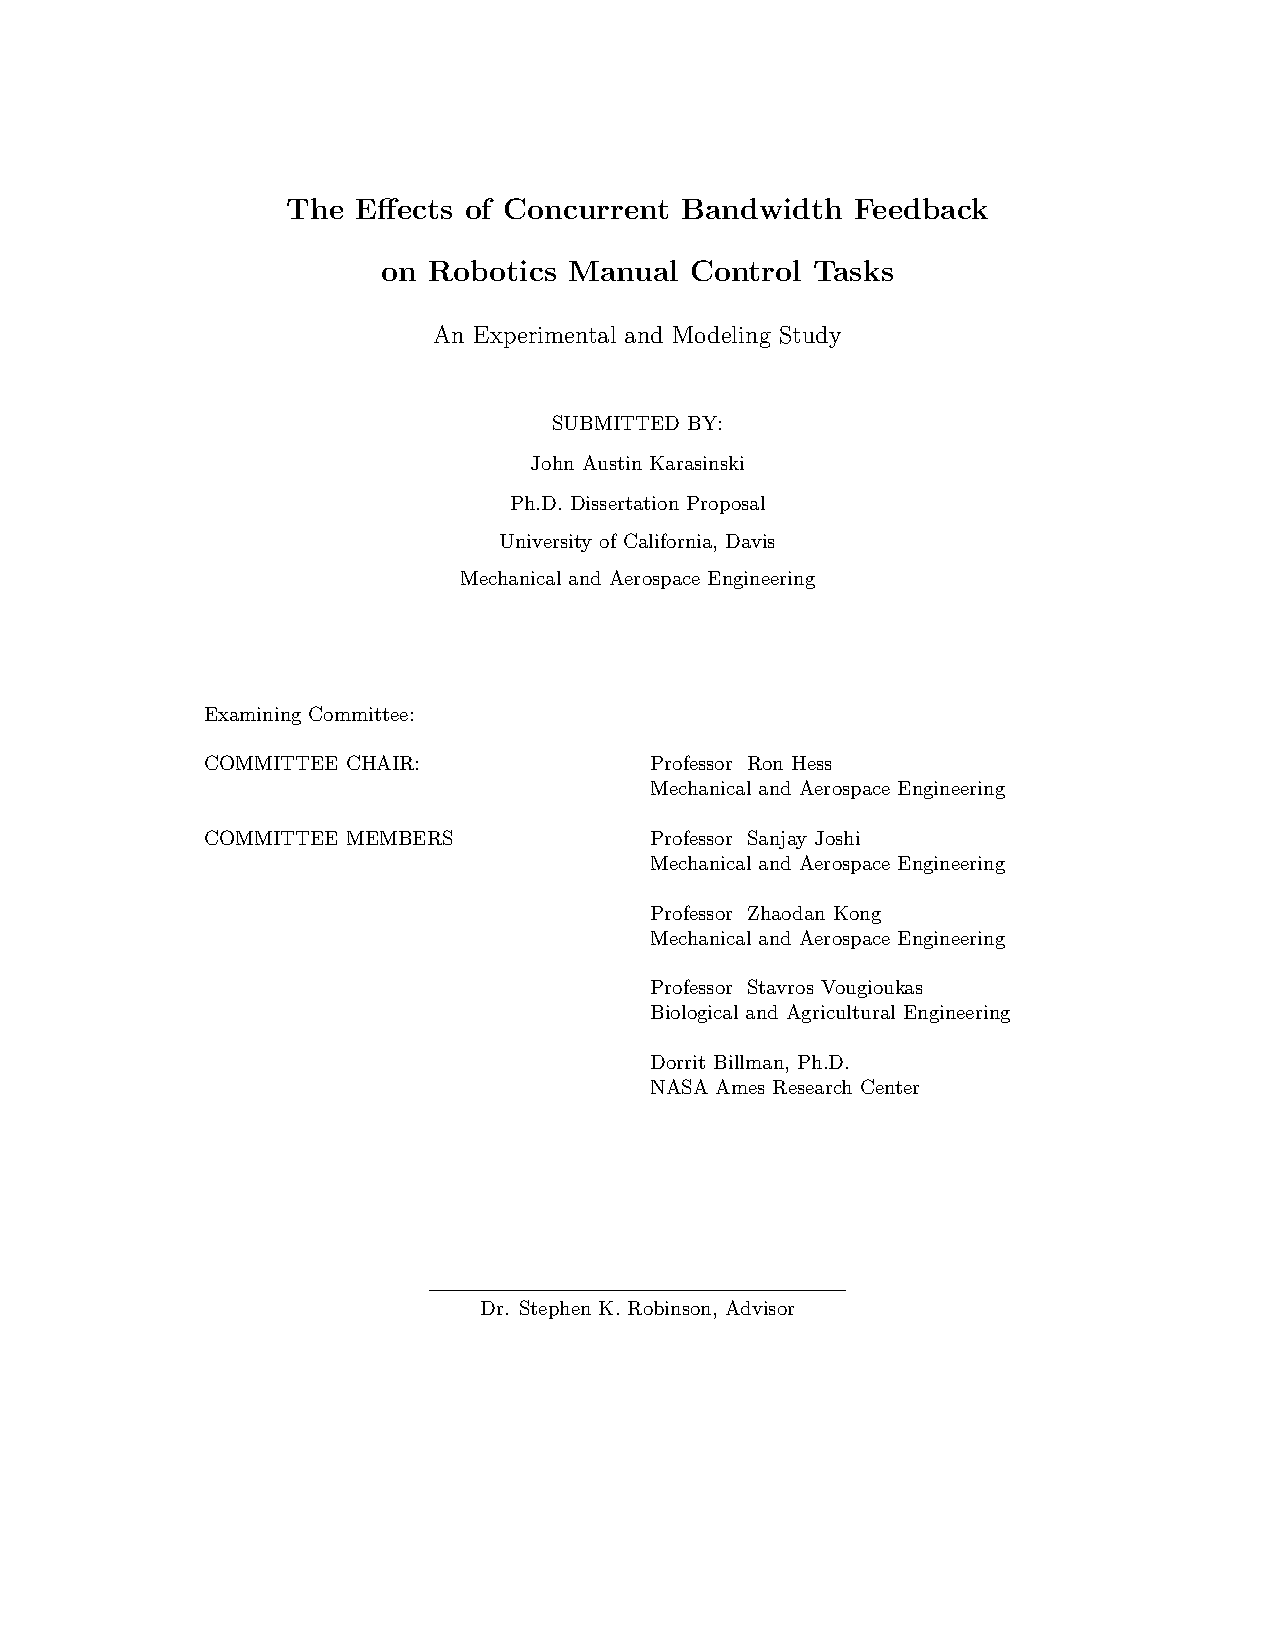
\includepdf{./pages/titlePage}
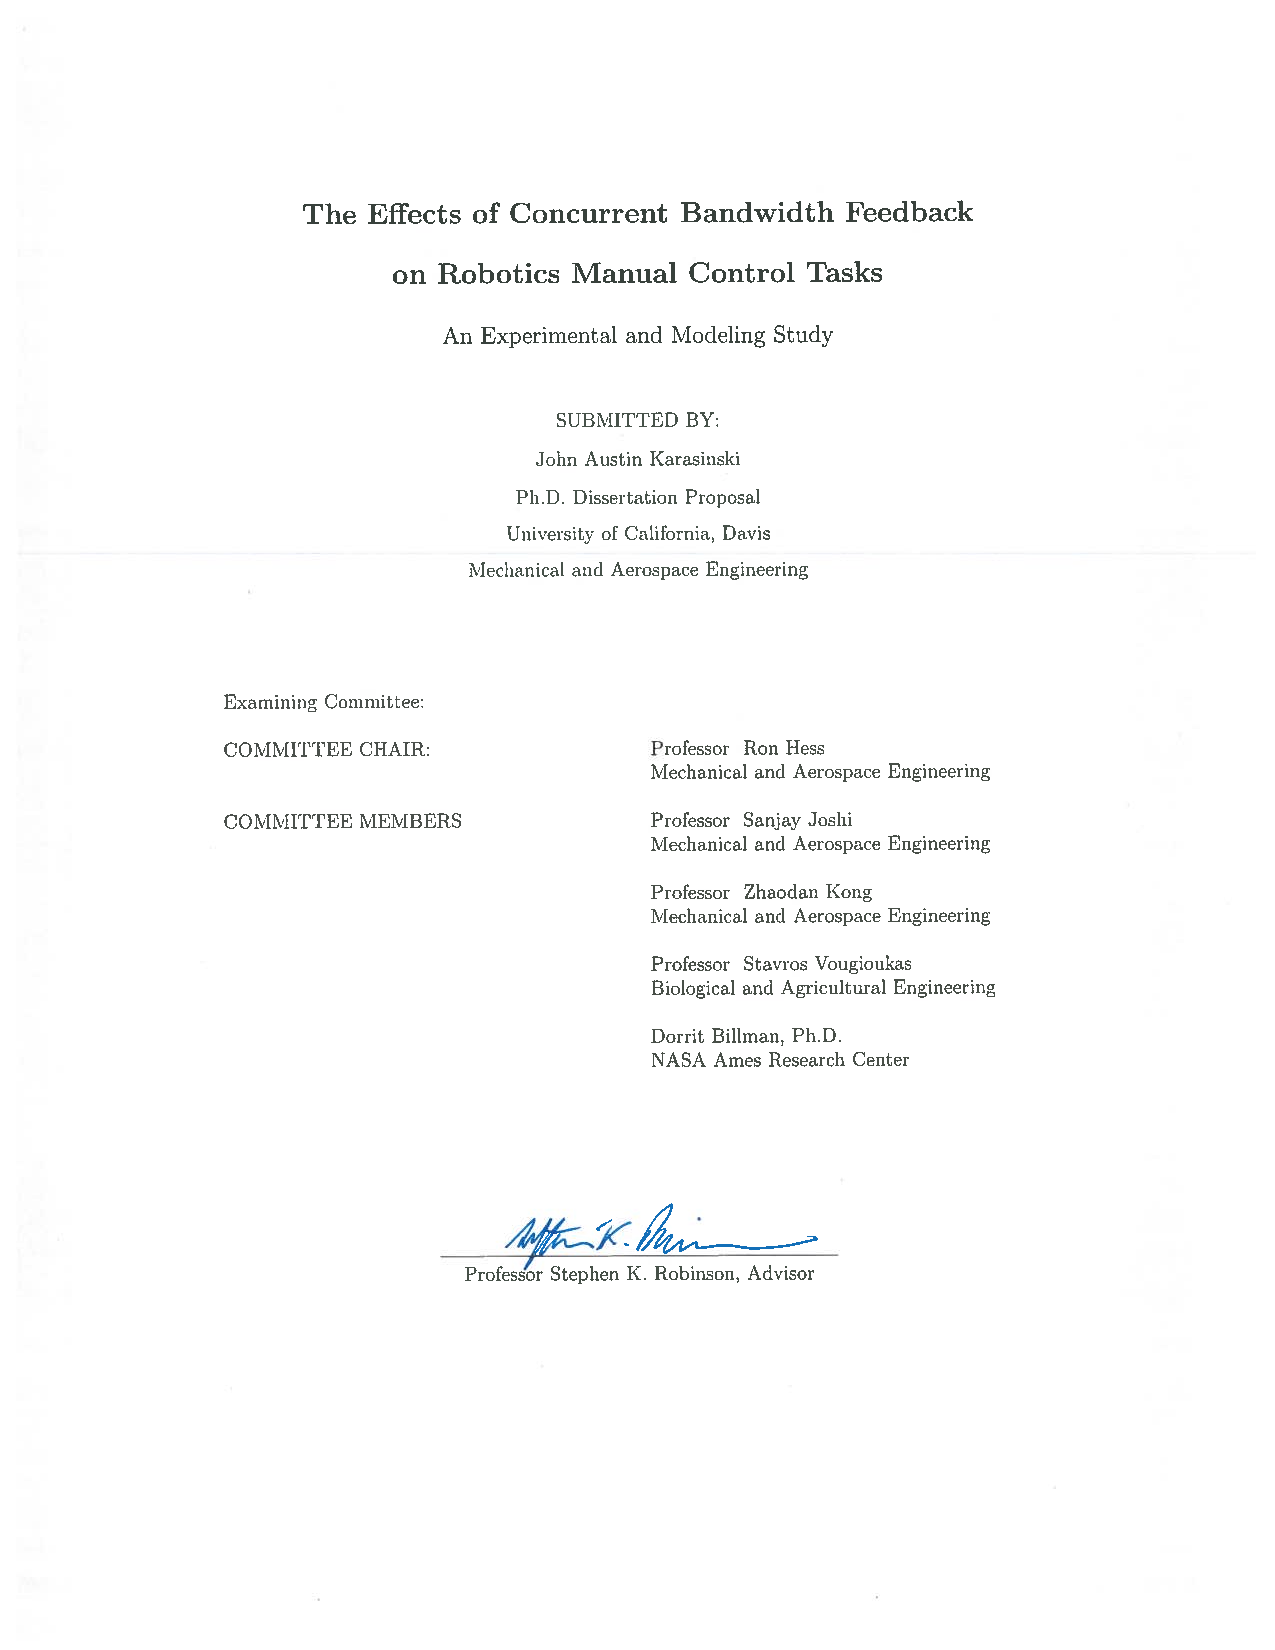
\includepdf[angle=90]{./pages/titlePageSigned}
\newpage \pagenumbering{roman}
\tableofcontents
\newpage \pagenumbering{arabic} \setcounter{page}{1}
\import{pages/}{problem}
\vspace{1em}
% \newpage
\import{pages/}{background}
\vspace{1em}
% \newpage
\import{pages/}{proposedresearch}
\vspace{1em}
% \newpage
\import{pages/}{risks}

\newpage
\bibliographystyle{ieeetr}
{\sffamily \footnotesize \setstretch{.5}
\bibliography{bib}
}
\end{document}
